\documentclass{article}\usepackage[]{graphicx}\usepackage[]{color}
%% maxwidth is the original width if it is less than linewidth
%% otherwise use linewidth (to make sure the graphics do not exceed the margin)
\makeatletter
\def\maxwidth{ %
  \ifdim\Gin@nat@width>\linewidth
    \linewidth
  \else
    \Gin@nat@width
  \fi
}
\makeatother

\definecolor{fgcolor}{rgb}{0.345, 0.345, 0.345}
\newcommand{\hlnum}[1]{\textcolor[rgb]{0.686,0.059,0.569}{#1}}%
\newcommand{\hlstr}[1]{\textcolor[rgb]{0.192,0.494,0.8}{#1}}%
\newcommand{\hlcom}[1]{\textcolor[rgb]{0.678,0.584,0.686}{\textit{#1}}}%
\newcommand{\hlopt}[1]{\textcolor[rgb]{0,0,0}{#1}}%
\newcommand{\hlstd}[1]{\textcolor[rgb]{0.345,0.345,0.345}{#1}}%
\newcommand{\hlkwa}[1]{\textcolor[rgb]{0.161,0.373,0.58}{\textbf{#1}}}%
\newcommand{\hlkwb}[1]{\textcolor[rgb]{0.69,0.353,0.396}{#1}}%
\newcommand{\hlkwc}[1]{\textcolor[rgb]{0.333,0.667,0.333}{#1}}%
\newcommand{\hlkwd}[1]{\textcolor[rgb]{0.737,0.353,0.396}{\textbf{#1}}}%
\let\hlipl\hlkwb

\usepackage{framed}
\makeatletter
\newenvironment{kframe}{%
 \def\at@end@of@kframe{}%
 \ifinner\ifhmode%
  \def\at@end@of@kframe{\end{minipage}}%
  \begin{minipage}{\columnwidth}%
 \fi\fi%
 \def\FrameCommand##1{\hskip\@totalleftmargin \hskip-\fboxsep
 \colorbox{shadecolor}{##1}\hskip-\fboxsep
     % There is no \\@totalrightmargin, so:
     \hskip-\linewidth \hskip-\@totalleftmargin \hskip\columnwidth}%
 \MakeFramed {\advance\hsize-\width
   \@totalleftmargin\z@ \linewidth\hsize
   \@setminipage}}%
 {\par\unskip\endMakeFramed%
 \at@end@of@kframe}
\makeatother

\definecolor{shadecolor}{rgb}{.97, .97, .97}
\definecolor{messagecolor}{rgb}{0, 0, 0}
\definecolor{warningcolor}{rgb}{1, 0, 1}
\definecolor{errorcolor}{rgb}{1, 0, 0}
\newenvironment{knitrout}{}{} % an empty environment to be redefined in TeX

\usepackage{alltt}

\title{Longer iterations}
\IfFileExists{upquote.sty}{\usepackage{upquote}}{}
\begin{document}








\begin{knitrout}
\definecolor{shadecolor}{rgb}{0.969, 0.969, 0.969}\color{fgcolor}\begin{kframe}
\begin{verbatim}
## [1] "initializing..."
\end{verbatim}
\end{kframe}
\end{knitrout}

In previous tests, Variational Bayes proved to be unreliable - each time I ran it, I got a different result. MCMC seemed to give posteriors for the learning rates that were uninformative. However, the effective sample size for MCMC turned out to be very small. Although the trace plots showed good evidence that chains had reached stability, I wanted to see whether we could get better results targetting an effective sample size of at least 10,000, as recommended by Kruschke (2014).

\section*{Method}

Because prior testing showed that across Analysis Repetitions for differing random seeds, there was very little change in the posteriors acquired when using MCMC, I only ran one repetition for MCMC. However, I ran 5 iterations for Variational Bayes, because prior testing showed vb was unreliable.


\begin{knitrout}
\definecolor{shadecolor}{rgb}{0.969, 0.969, 0.969}\color{fgcolor}
\begin{tabular}{l|l|r|r}
\hline
EstimationMethod & Model & Group & N\\
\hline
MCMC & double\_update\_notrialpost & 2 & 1\\
\hline
MCMC & double\_update\_notrialpost & 3 & 1\\
\hline
MCMC & double\_update\_rpo\_repeated\_runs\_notrialpost & 2 & 1\\
\hline
MCMC & double\_update\_rpo\_repeated\_runs\_notrialpost & 3 & 1\\
\hline
variationalbayes & double\_update\_notrialpost & 2 & 5\\
\hline
variationalbayes & double\_update\_notrialpost & 3 & 5\\
\hline
variationalbayes & double\_update\_rpo\_repeated\_runs\_notrialpost & 2 & 5\\
\hline
variationalbayes & double\_update\_rpo\_repeated\_runs\_notrialpost & 3 & 5\\
\hline
\end{tabular}


\end{knitrout}


\section*{Results}





Estimations for Punishment data appeared to differ somewhat when both runs and when reward data was added, as we'd expect.


\subsection*{VB}
Is Variational Bayes just as unreliable as previously?

\begin{knitrout}
\definecolor{shadecolor}{rgb}{0.969, 0.969, 0.969}\color{fgcolor}
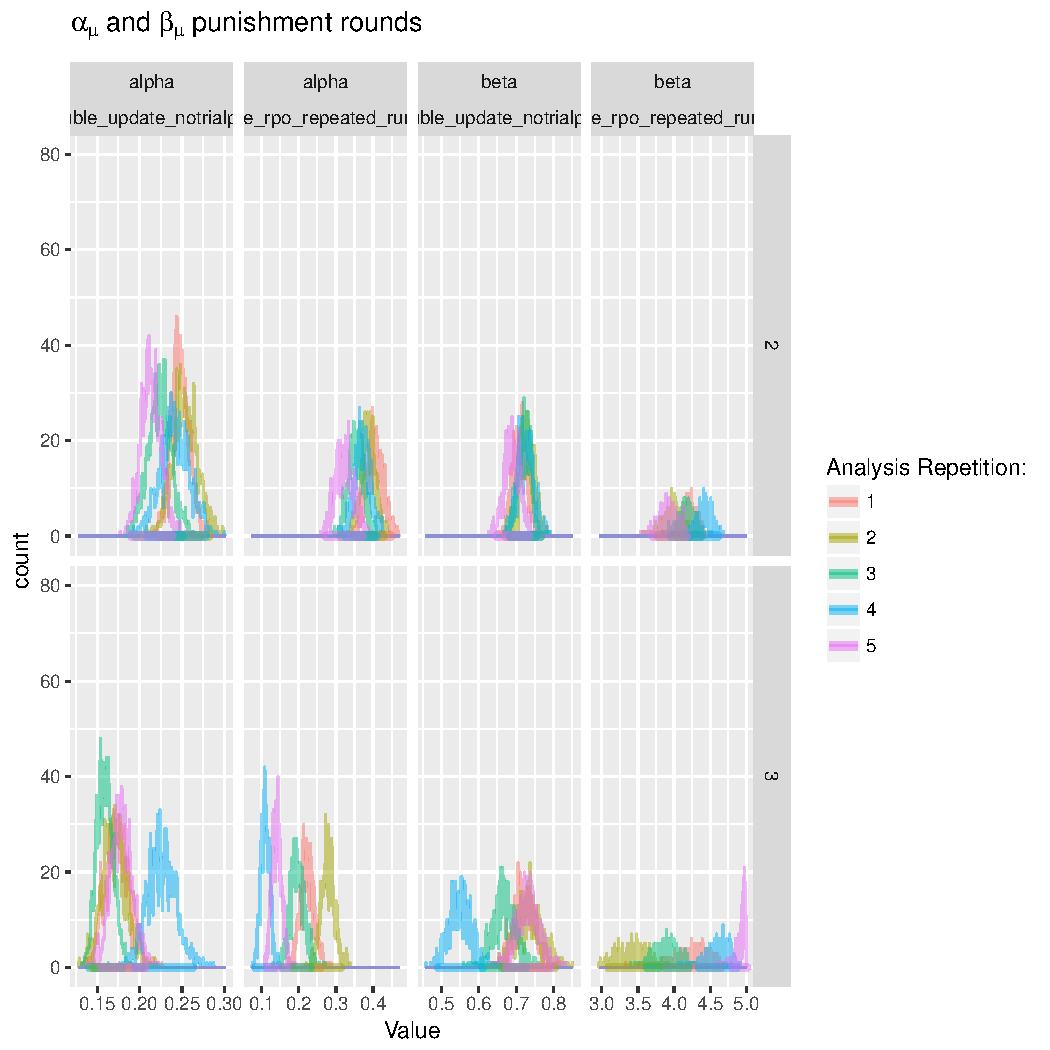
\includegraphics[width=\maxwidth]{figure/unnamed-chunk-6-1} 
\begin{kframe}\begin{verbatim}
## [1] 0.228005 0.270512
## [1] 0.224073 0.281191
## [1] 0.195218 0.249667
## [1] 0.210205 0.276934
## [1] 0.191073 0.237313
## [1] 0.361738 0.447002
## [1] 0.351804 0.426227
## [1] 0.316253 0.399951
## [1] 0.329627 0.407424
## [1] 0.275549 0.369449
## [1] 0.675388 0.748101
## [1] 0.685730 0.763173
## [1] 0.685334 0.751036
## [1] 0.686809 0.764552
## [1] 0.650024 0.732362
## [1] 4.05039 4.36505
## [1] 3.78599 4.20328
## [1] 3.96845 4.35992
## [1] 4.24411 4.59813
## [1] 3.71367 4.16176
## [1] 0.147886 0.202997
## [1] 0.146002 0.202097
## [1] 0.141775 0.178637
## [1] 0.195506 0.261815
## [1] 0.155323 0.206250
## [1] 0.186071 0.255631
## [1] 0.239221 0.310884
## [1] 0.158204 0.229507
## [1] 0.0860459 0.1326850
## [1] 0.117391 0.166601
## [1] 0.671173 0.782499
## [1] 0.664909 0.801076
## [1] 0.612258 0.724670
## [1] 0.493028 0.608738
## [1] 0.676415 0.791156
## [1] 3.88932 4.63673
## [1] 3.10762 3.78257
## [1] 3.63546 4.18451
## [1] 4.35460 4.85259
## [1] 4.81979 4.99789
\end{verbatim}
\end{kframe}
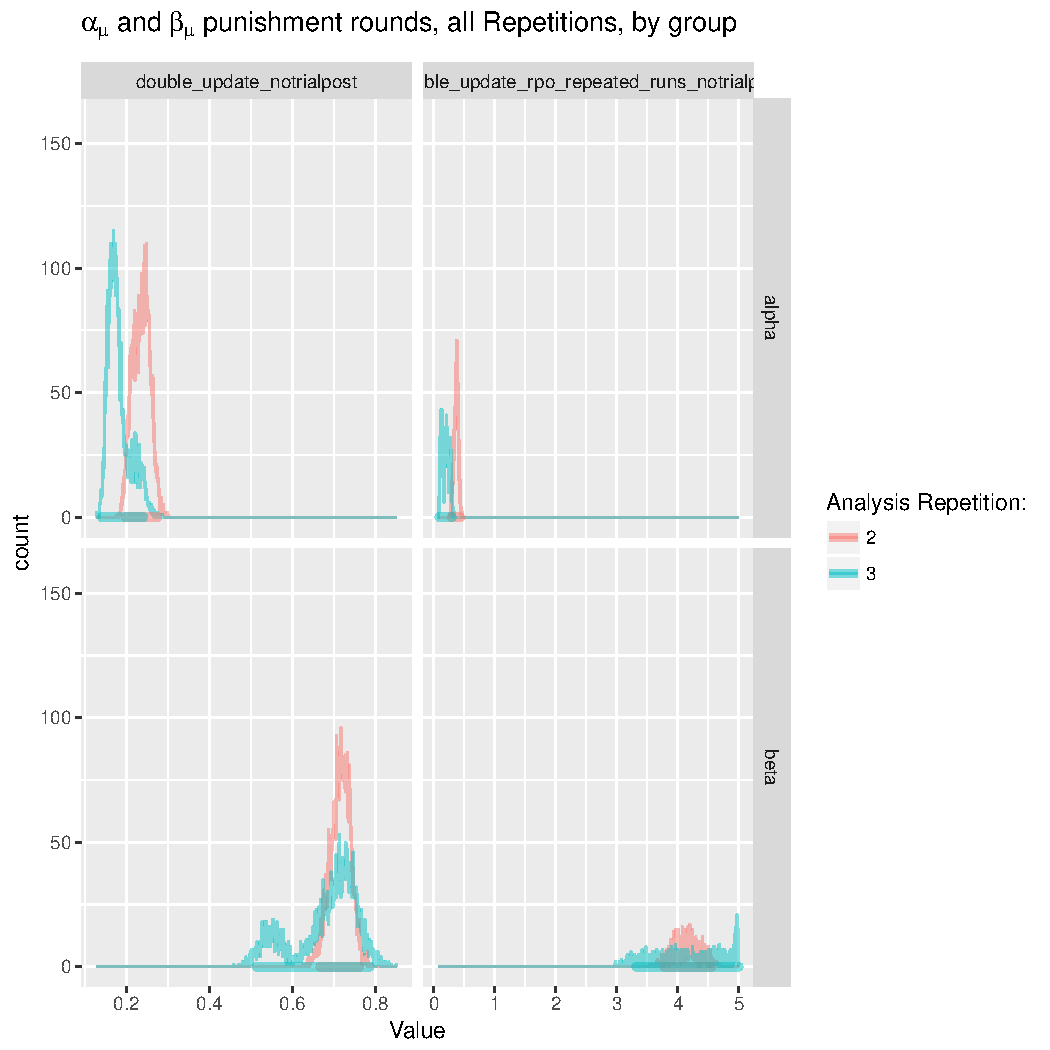
\includegraphics[width=\maxwidth]{figure/unnamed-chunk-6-2} 
\begin{kframe}\begin{verbatim}
## [1] 0.198647 0.274813
## [1] 0.141382 0.240055
## [1] 0.298041 0.432642
## [1] 0.0930779 0.2944810
## [1] 0.667474 0.761013
## [1] 0.514389 0.786345
## [1] 3.78069 4.55038
## [1] 3.32090 4.99603
\end{verbatim}
\end{kframe}
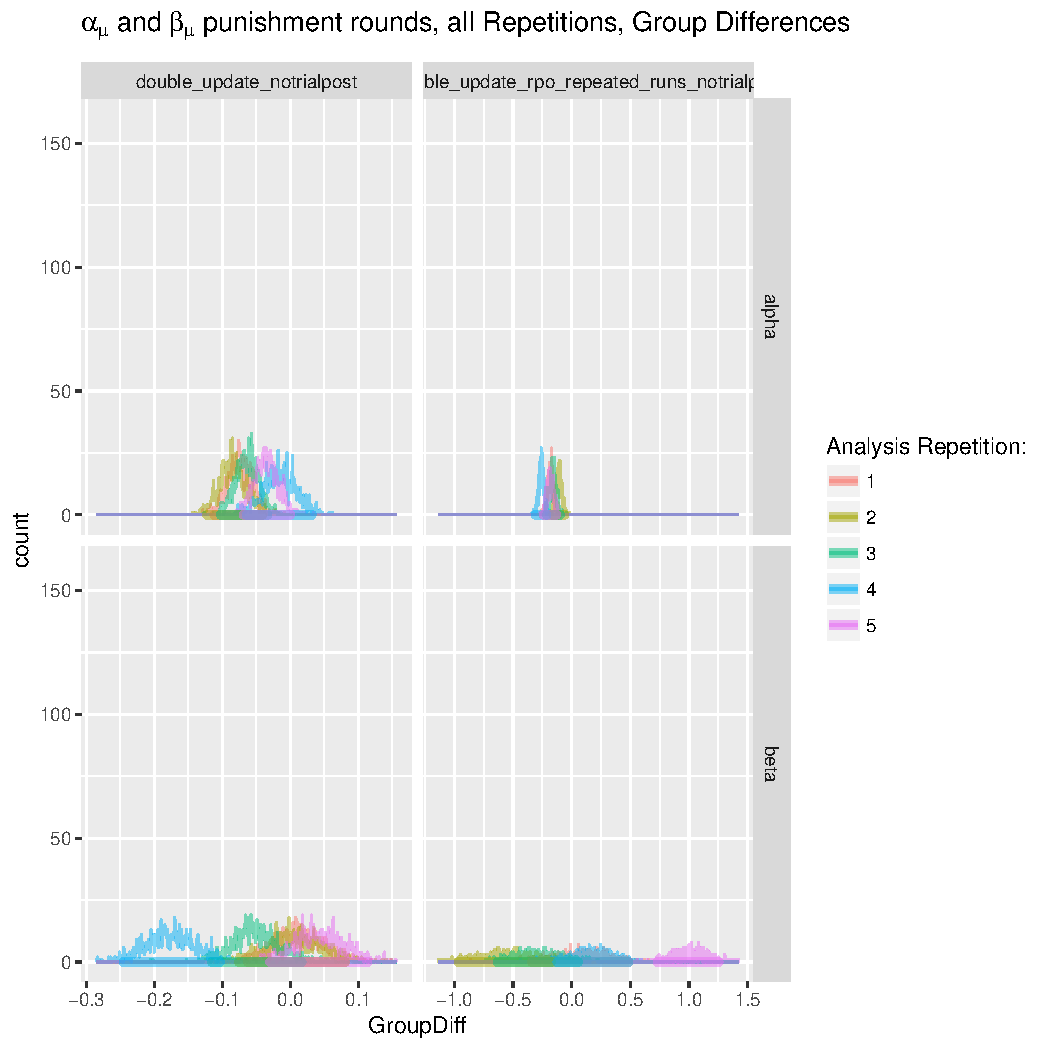
\includegraphics[width=\maxwidth]{figure/unnamed-chunk-6-3} 
\begin{kframe}\begin{verbatim}
## [1] -0.111649 -0.041202
## [1] -0.122359 -0.041840
## [1] -0.102016 -0.034058
## [1] -0.064533  0.031441
## [1] -0.068952 -0.000486
## [1] -0.237782 -0.122736
## [1] -0.156909 -0.061710
## [1] -0.209523 -0.100410
## [1] -0.307654 -0.216919
## [1] -0.235936 -0.132460
## [1] -0.062150  0.079766
## [1] -0.075279  0.080361
## [1] -0.115202  0.016577
## [1] -0.245408 -0.103892
## [1] -0.029594  0.113224
## [1] -0.33773  0.48099
## [1] -0.96143 -0.17661
## [1] -0.63106  0.05251
## [1] -0.12224  0.48272
## [1] 0.73405 1.25150
\end{verbatim}
\end{kframe}
\end{knitrout}

Unfortunately, Variational Bayes stil does not seem to be sitting on consistent estimations. Not only do Analysis Repetition HDIs not even overlap, but group differences sit across the 0 point in inconsistent ways.

\subsection*{MCMC}

Are our MCMC estimates any use?
\subsubsection*{Results}
\begin{knitrout}
\definecolor{shadecolor}{rgb}{0.969, 0.969, 0.969}\color{fgcolor}
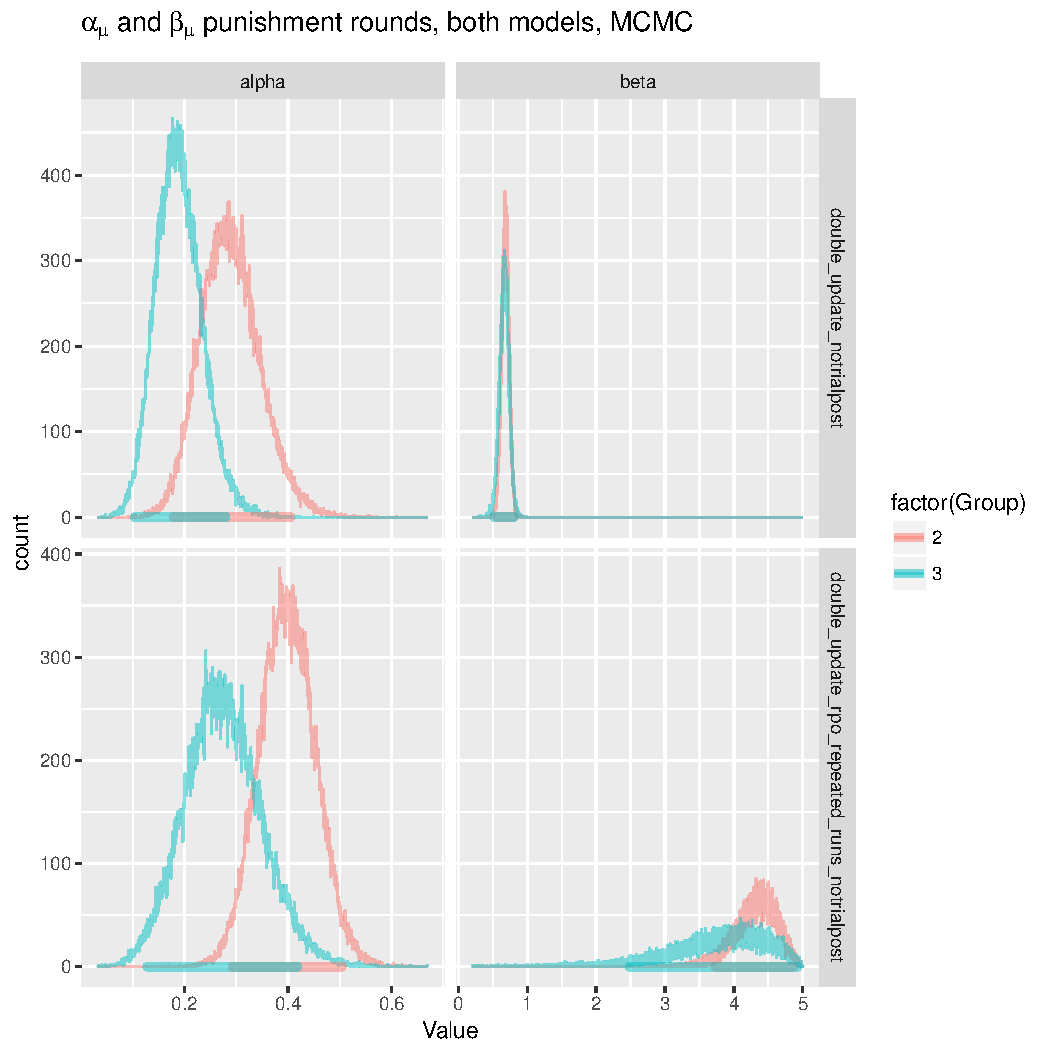
\includegraphics[width=\maxwidth]{figure/unnamed-chunk-7-1} 
\begin{kframe}\begin{verbatim}
## [1] 0.1799103 0.4041590
## [1] 0.1044252 0.2791976
## [1] 0.5760161 0.7941830
## [1] 0.5293238 0.8039285
## [1] 0.2928371 0.5035468
## [1] 0.1284228 0.4178588
## [1] 3.730358 4.856850
## [1] 2.48634 4.92266
\end{verbatim}
\end{kframe}
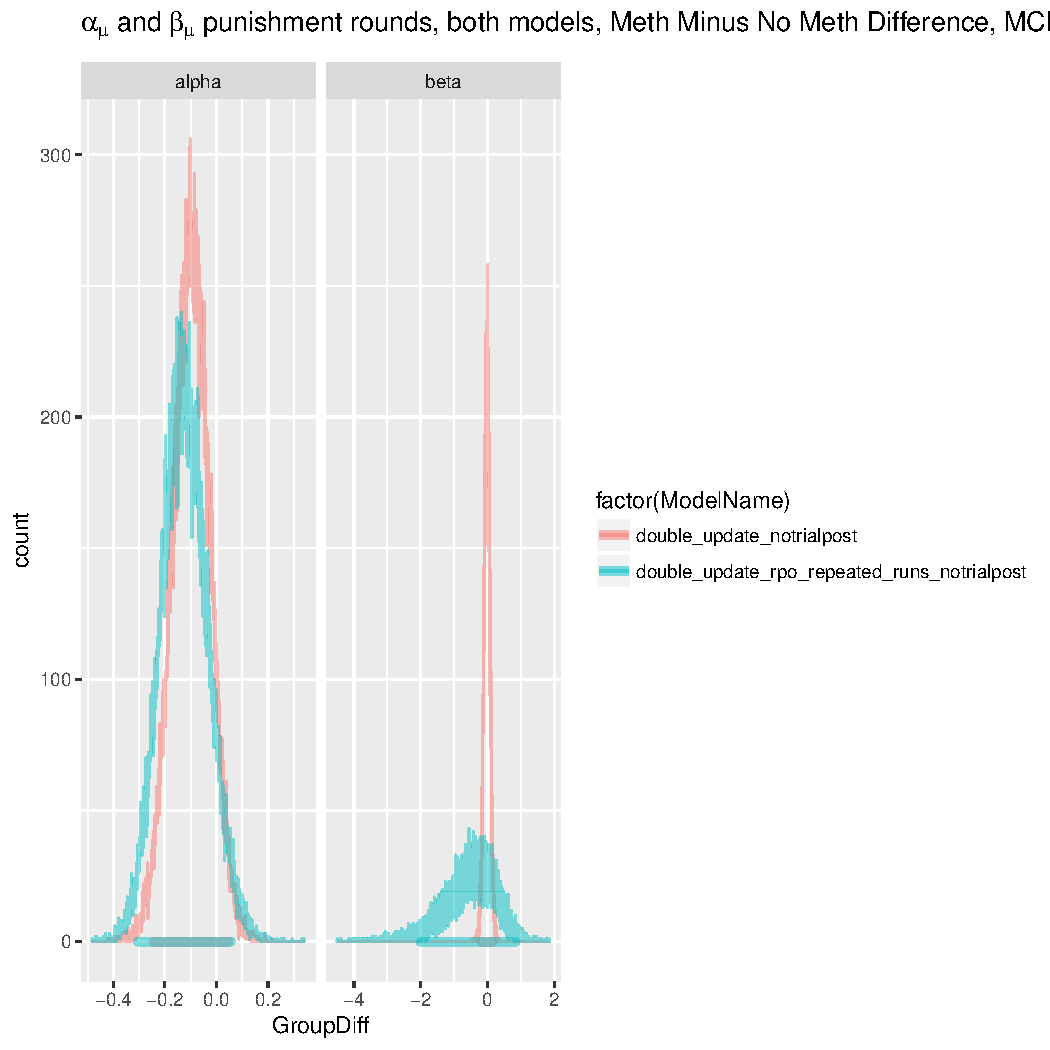
\includegraphics[width=\maxwidth]{figure/unnamed-chunk-7-2} 
\begin{kframe}\begin{verbatim}
## [1] -0.2411440  0.0451379
## [1] -0.30478558  0.05571068
## [1] -0.1883593  0.1597689
## [1] -2.0052018  0.8355794
\end{verbatim}
\end{kframe}
\end{knitrout}

Unfortunately, at least for this statistic, we don't seem to be able to distinguish between groups. What about for just the repeated runs model with Reward and Punishment?

\begin{knitrout}
\definecolor{shadecolor}{rgb}{0.969, 0.969, 0.969}\color{fgcolor}
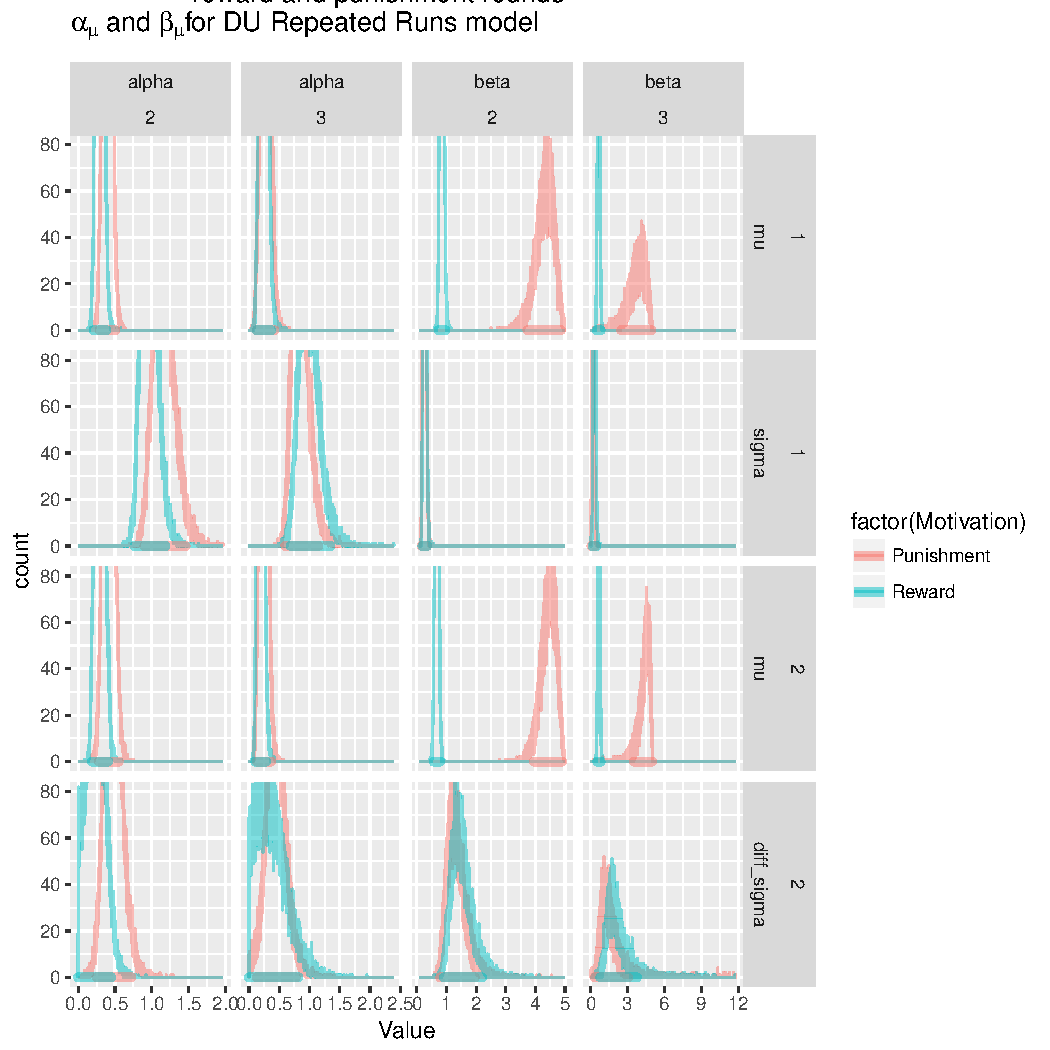
\includegraphics[width=\maxwidth]{figure/unnamed-chunk-8-1} 
\begin{kframe}\begin{verbatim}
## [1] 0.2928371 0.5035468
## [1] 0.2082229 0.3814867
## [1] 0.1284228 0.4178588
## [1] 0.1301943 0.3661932
## [1] 3.730358 4.856850
## [1] 0.7357677 0.9676815
## [1] 2.48634 4.92266
## [1] 0.4859561 0.8030683
## [1] 0.9000871 1.4590425
## [1] 0.767198 1.186891
## [1] 0.5998997 1.1444645
## [1] 0.6906578 1.3451125
## [1] 0.1660095 0.3404435
## [1] 0.1850241 0.3474949
## [1] 0.04591472 0.33144112
## [1] 0.1441056 0.4612514
## [1] 0.2811134 0.5512065
## [1] 0.1858282 0.4043800
## [1] 0.1290673 0.3613335
## [1] 0.1057864 0.2812338
## [1] 3.946701 4.897566
## [1] 0.5692587 0.7796828
## [1] 3.517272 4.998446
## [1] 0.5274377 0.7988943
## [1] 0.2521776 0.7249430
## [1] 5.280459e-05 4.487905e-01
## [1] 0.1289889 0.7734066
## [1] 5.732574e-05 8.186682e-01
## [1] 0.7894919 1.9540100
## [1] 0.918375 2.195202
## [1] 0.333266 3.028804
## [1] 0.777374 3.749612
\end{verbatim}
\end{kframe}
\end{knitrout}

Here, the model does seem to show evidence of *inverse temperature* but not *learning rate*. This might be interesting.

\begin{knitrout}
\definecolor{shadecolor}{rgb}{0.969, 0.969, 0.969}\color{fgcolor}
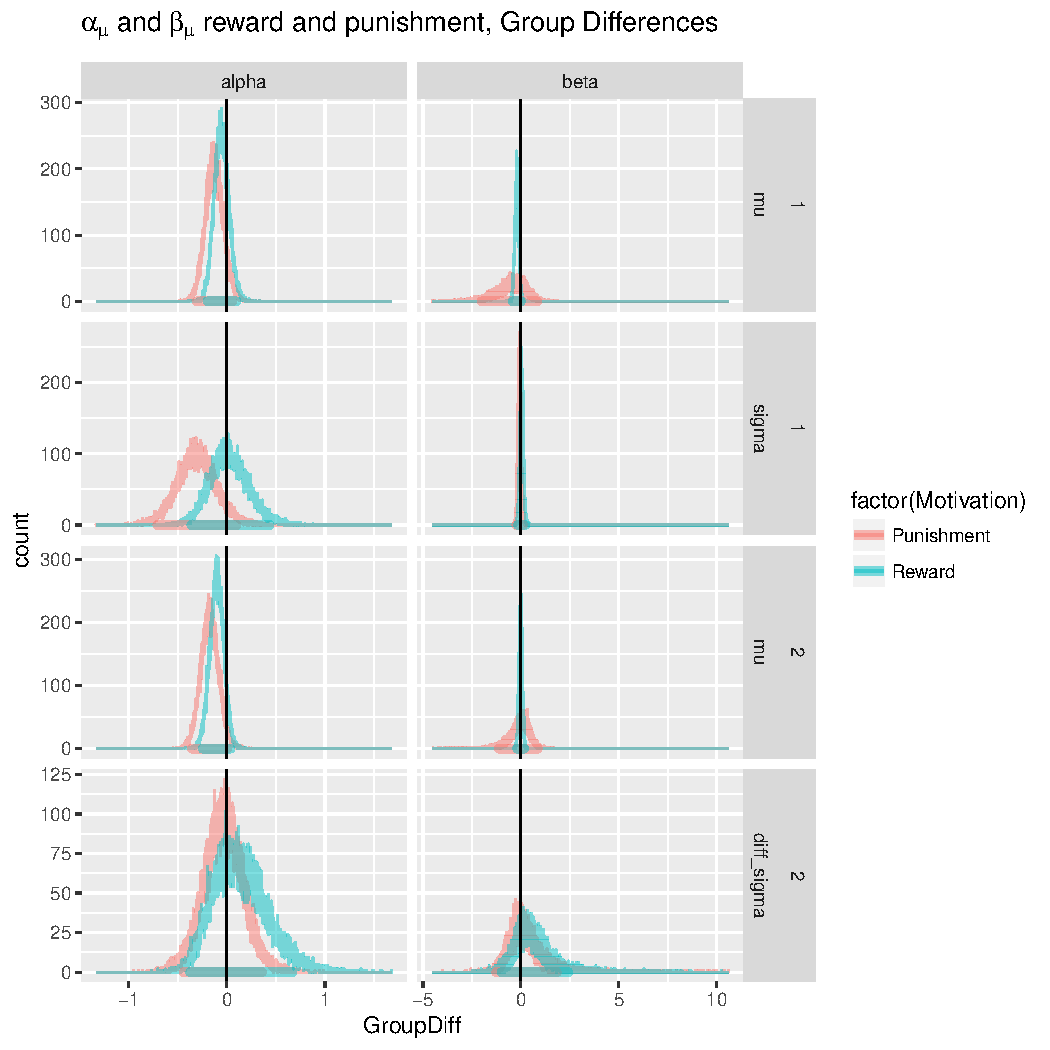
\includegraphics[width=\maxwidth]{figure/unnamed-chunk-9-1} 
\begin{kframe}\begin{verbatim}
## [1] -0.30478558  0.05571068
## [1] -0.19451082  0.09924172
## [1] -2.0052018  0.8355794
## [1] -0.397614249 -0.002657135
## [1] -0.70556734  0.09620654
## [1] -0.3597393  0.4320685
## [1] -0.2265336  0.1046957
## [1] -0.1385795  0.2175001
## [1] -0.356055456  0.002833918
## [1] -0.24480219  0.03759113
## [1] -1.1163552  0.8610196
## [1] -0.1848512  0.1583106
## [1] -0.4368147  0.3573772
## [1] -0.3715092  0.6657589
## [1] -1.254109  1.830467
## [1] -0.9782443  2.4142420
\end{verbatim}
\end{kframe}
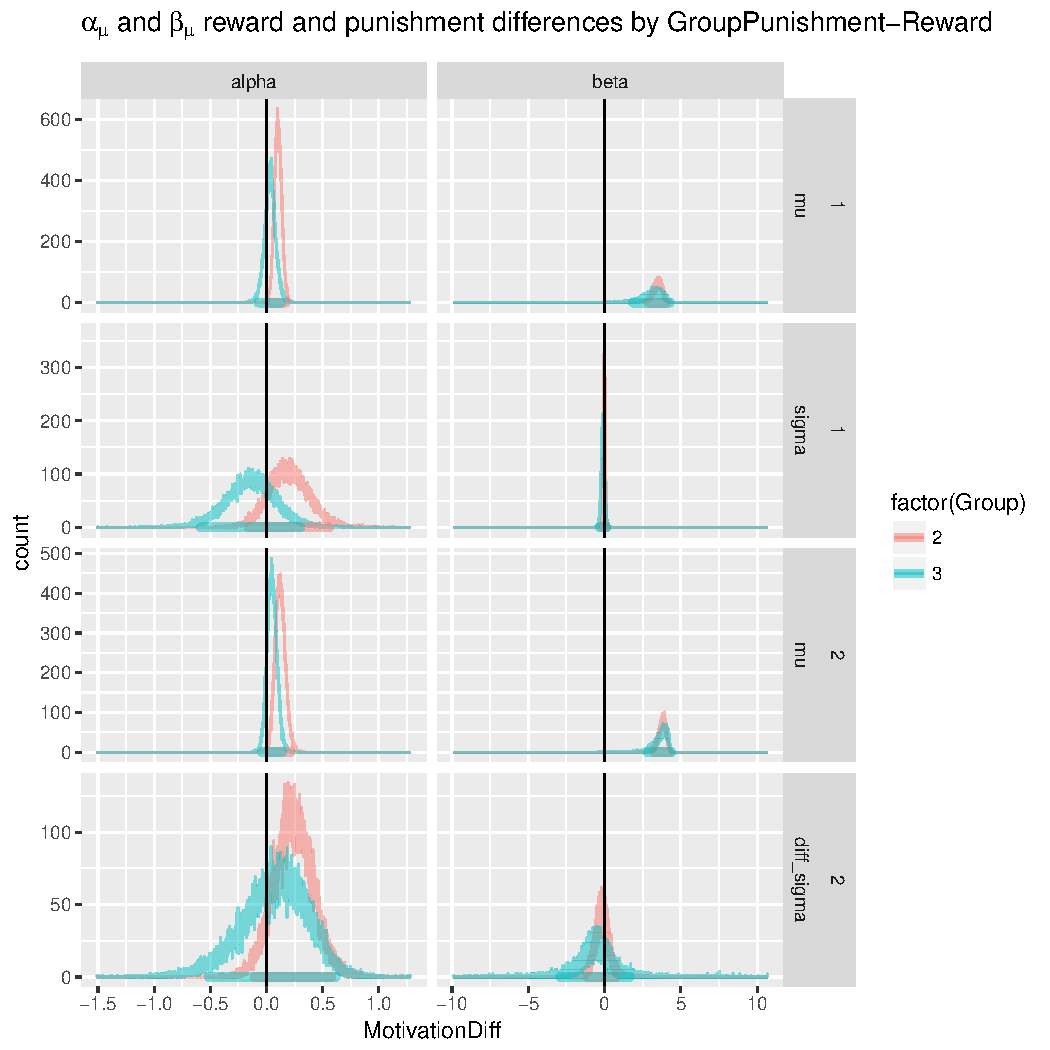
\includegraphics[width=\maxwidth]{figure/unnamed-chunk-9-2} 
\begin{kframe}\begin{verbatim}
## [1] 0.03993872 0.16887087
## [1] -0.07085384  0.12928783
## [1] 2.890878 4.010670
## [1] 1.856131 4.264327
## [1] -0.1556246  0.5579511
## [1] -0.5838224  0.2973300
## [1] -0.1302542  0.1111737
## [1] -0.3214038  0.1049233
## [1] 0.03410208 0.21420971
## [1] -0.03780864  0.13697689
## [1] 3.283022 4.227310
## [1] 2.840951 4.355423
## [1] -0.1050331  0.5782097
## [1] -0.5113432  0.6170295
## [1] -1.1220467  0.7148964
## [1] -2.900168  1.638450
\end{verbatim}
\end{kframe}
\end{knitrout}

Once again, there do not appear to be any differences between our two groups. Consistent across groups, we do see potentially large differences in Reward and Punishment in inverse temperature, though not learning rate.

But can we trust these values?

\subsubsection*{Diagnostics: Efficiency}

\begin{knitrout}
\definecolor{shadecolor}{rgb}{0.969, 0.969, 0.969}\color{fgcolor}
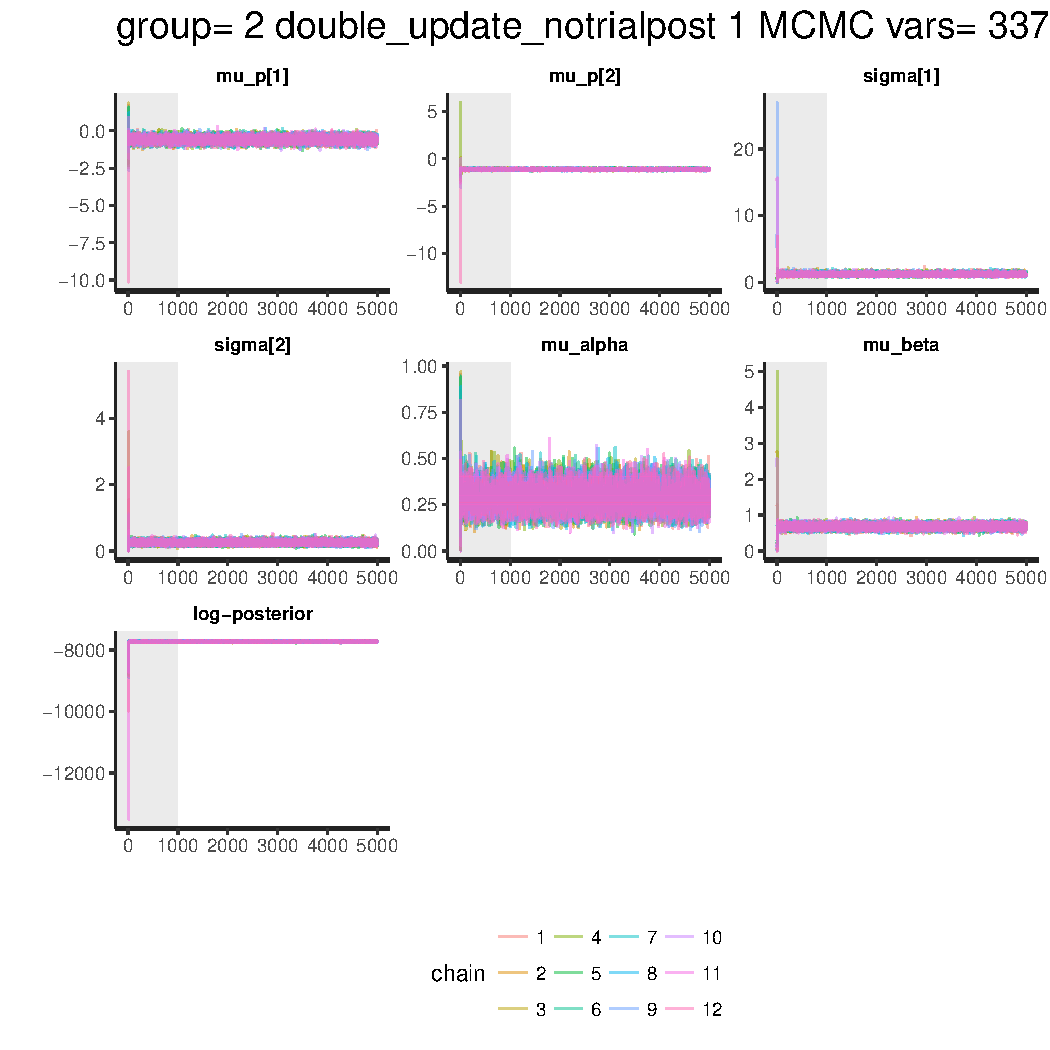
\includegraphics[width=\maxwidth]{figure/unnamed-chunk-10-1} 

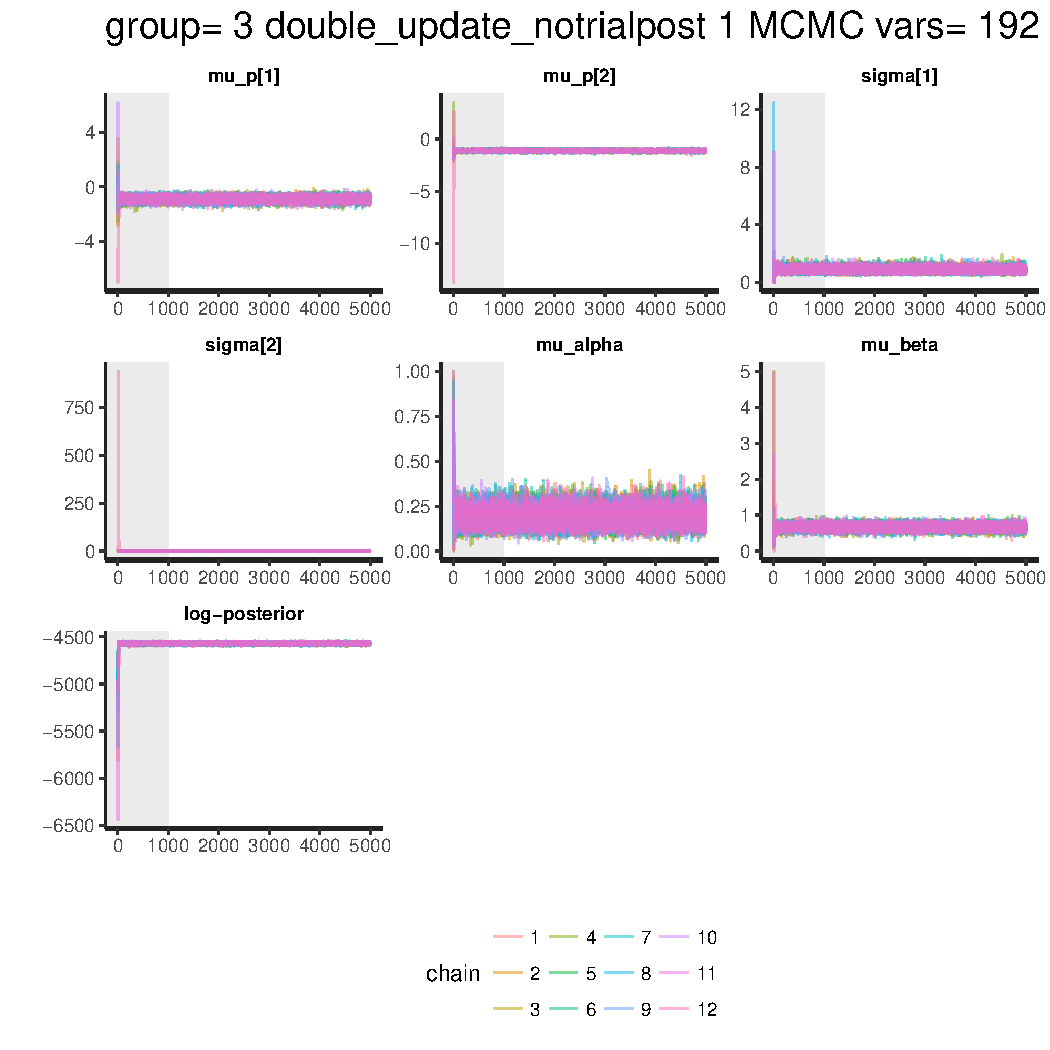
\includegraphics[width=\maxwidth]{figure/unnamed-chunk-10-2} 

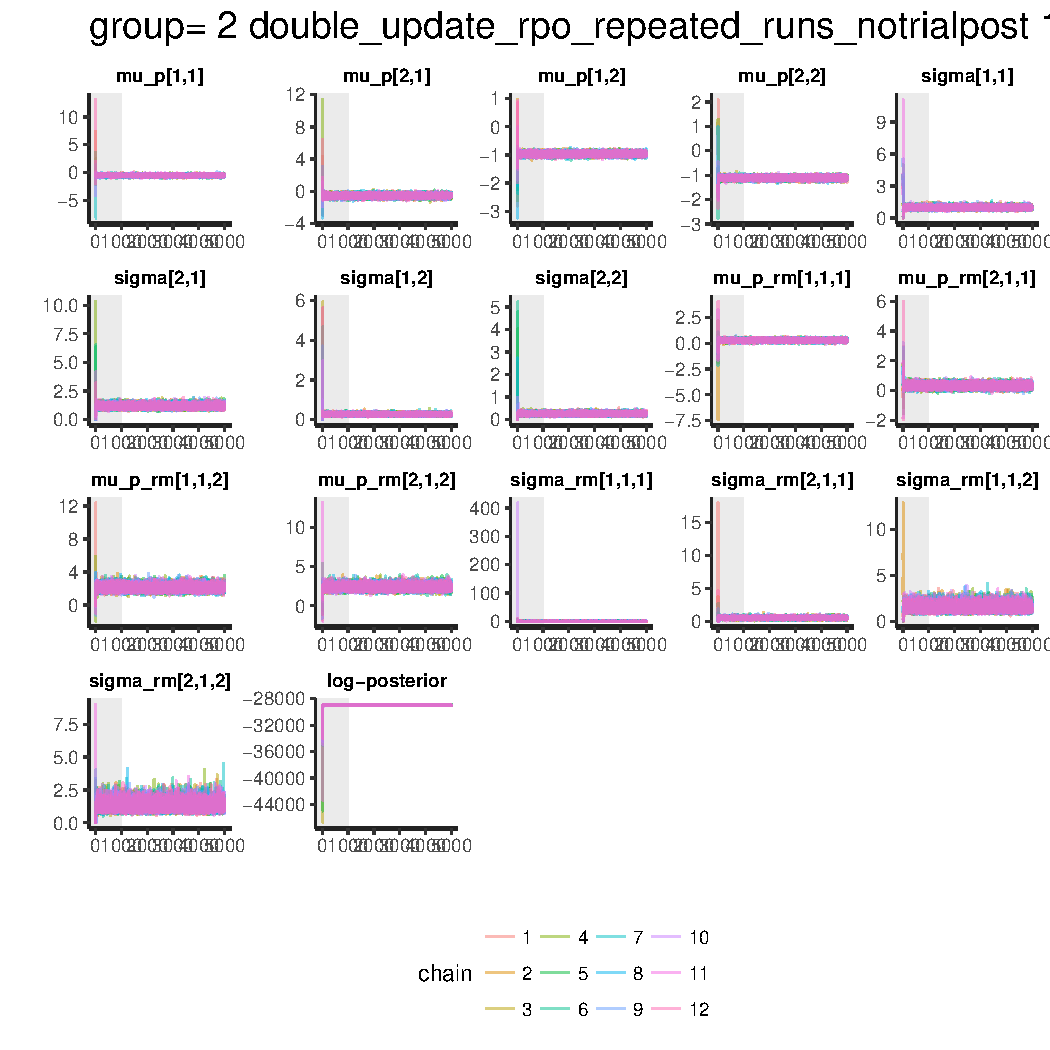
\includegraphics[width=\maxwidth]{figure/unnamed-chunk-10-3} 

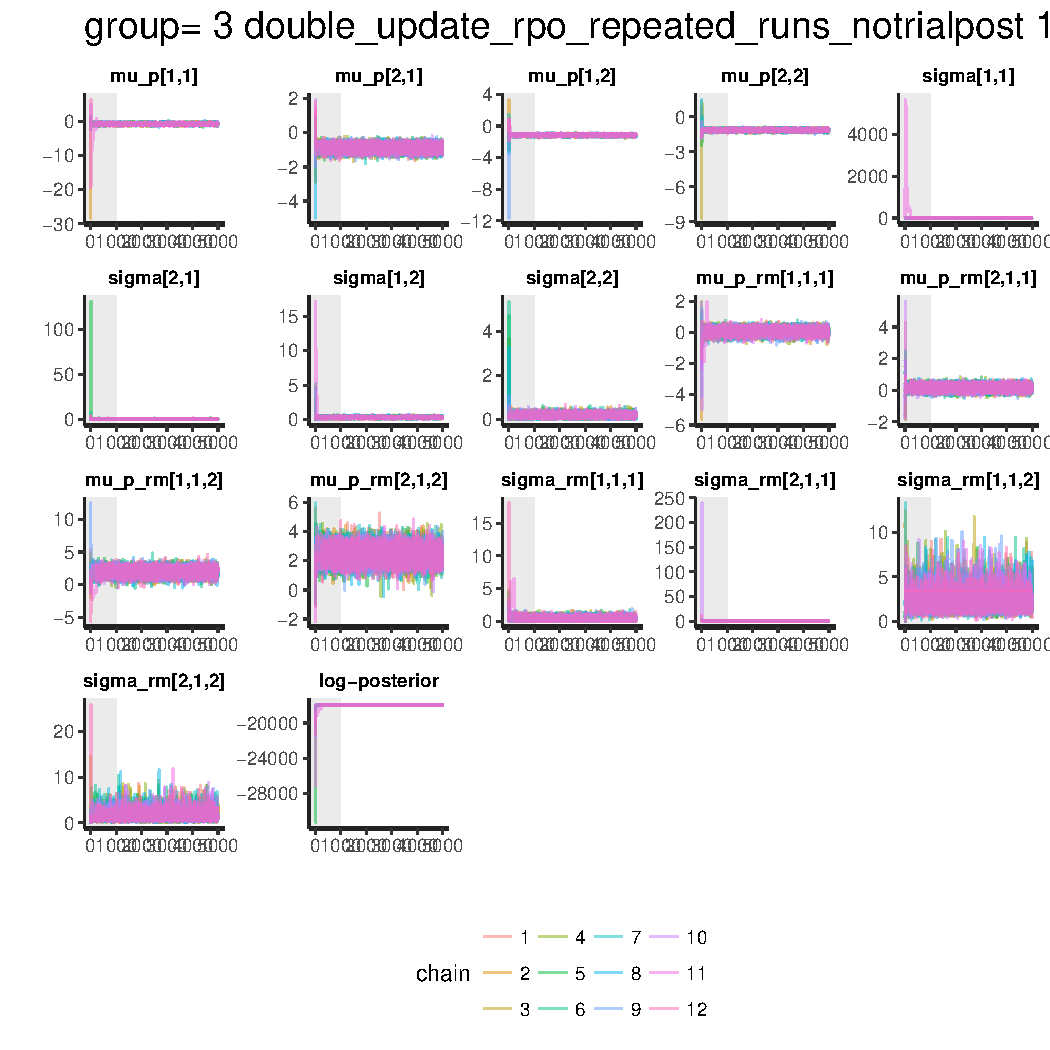
\includegraphics[width=\maxwidth]{figure/unnamed-chunk-10-4} 

\end{knitrout}

Once again, the traceplots indicate good representativeness: these values have tended to converge very quickly, albeit on fairly large intervals.

\begin{knitrout}
\definecolor{shadecolor}{rgb}{0.969, 0.969, 0.969}\color{fgcolor}\begin{kframe}


{\ttfamily\noindent\bfseries\color{errorcolor}{\#\# Error in xy.coords(x, y, xlabel, ylabel, log): 'x' and 'y' lengths differ}}\end{kframe}
\end{knitrout}

Monte Carlo Standard Error:

\begin{knitrout}
\definecolor{shadecolor}{rgb}{0.969, 0.969, 0.969}\color{fgcolor}
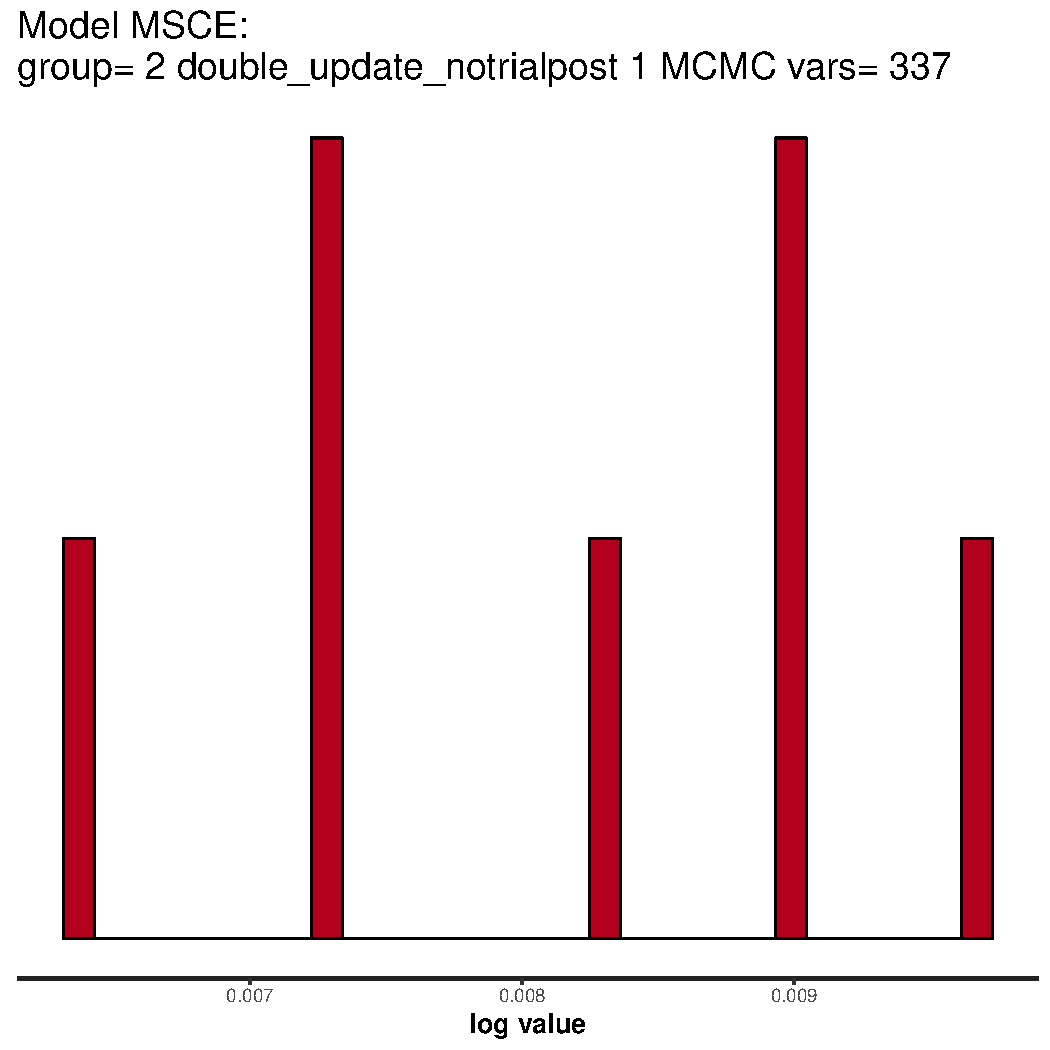
\includegraphics[width=\maxwidth]{figure/unnamed-chunk-12-1} 

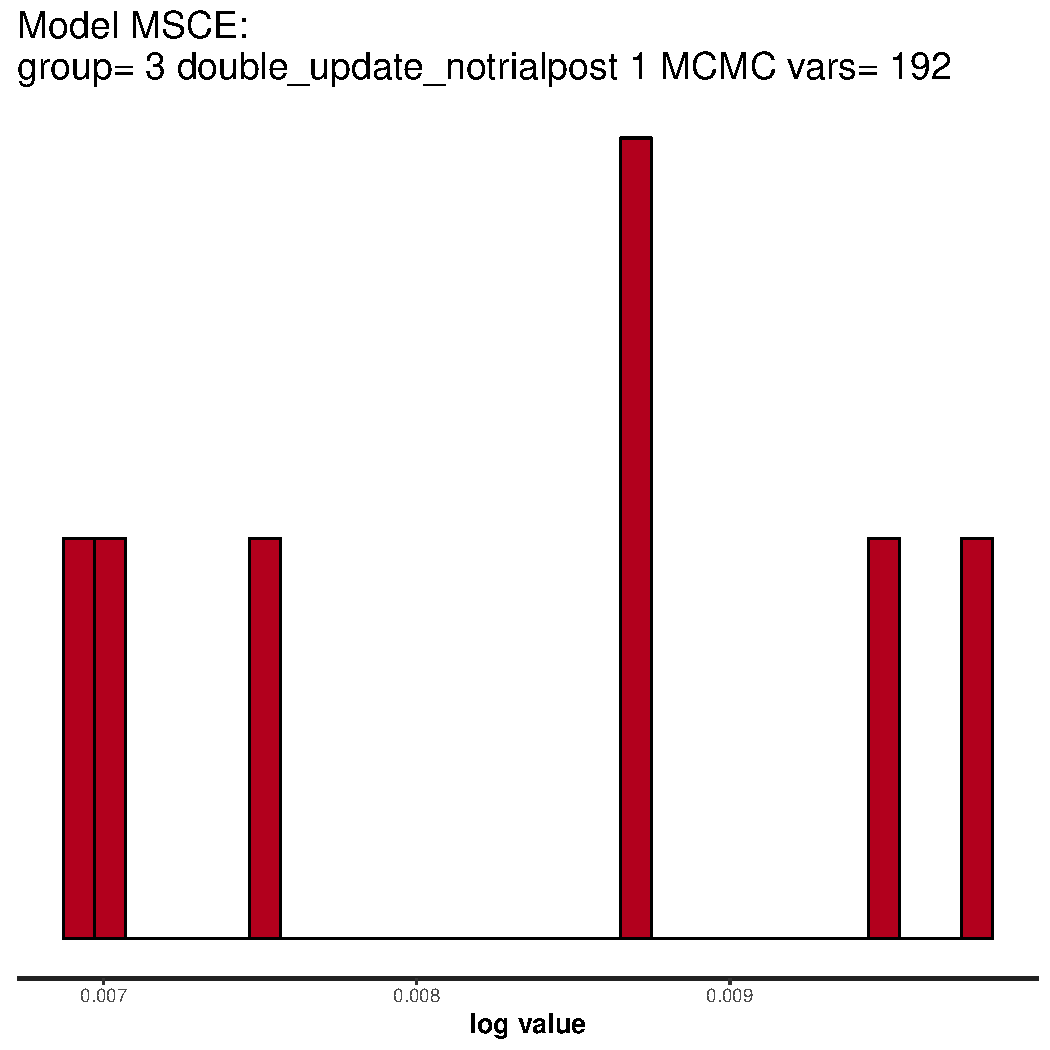
\includegraphics[width=\maxwidth]{figure/unnamed-chunk-12-2} 

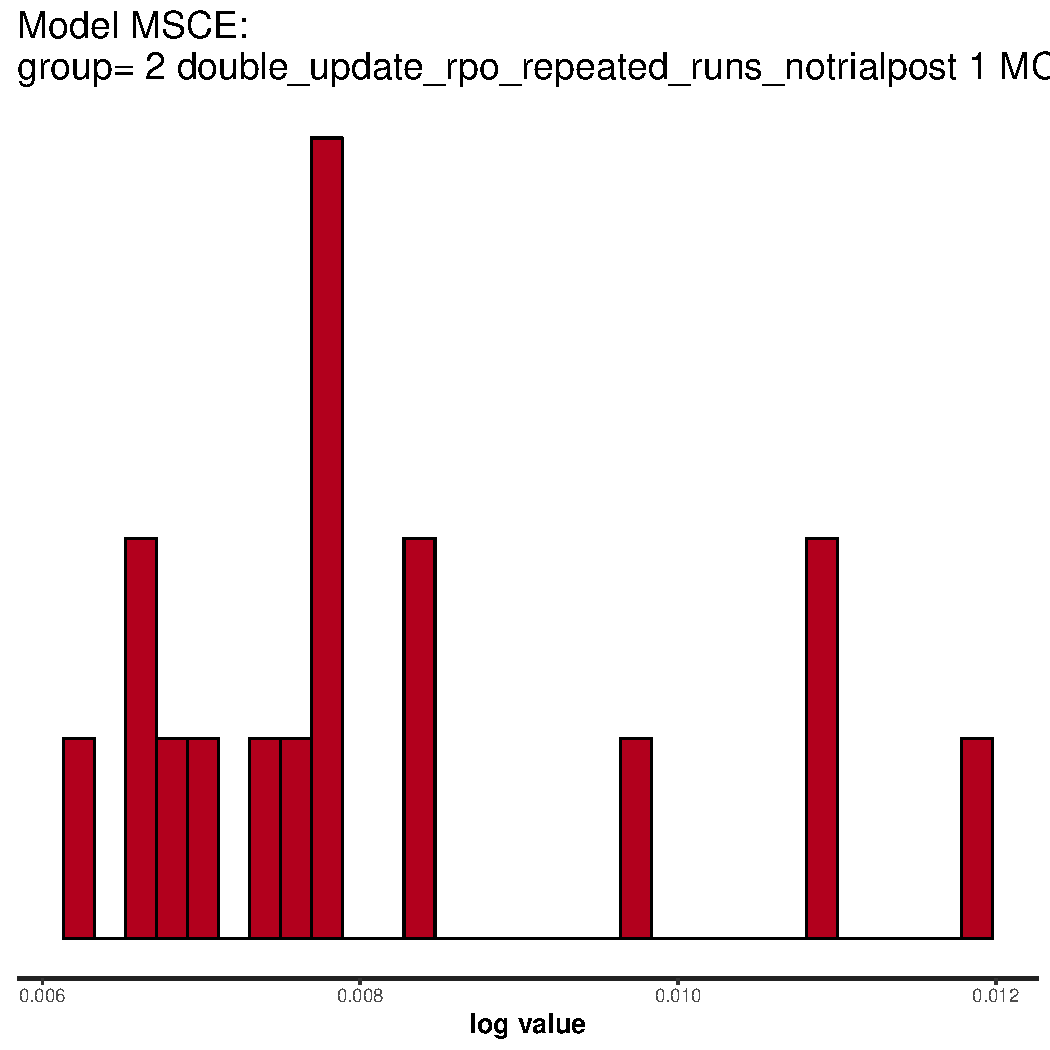
\includegraphics[width=\maxwidth]{figure/unnamed-chunk-12-3} 

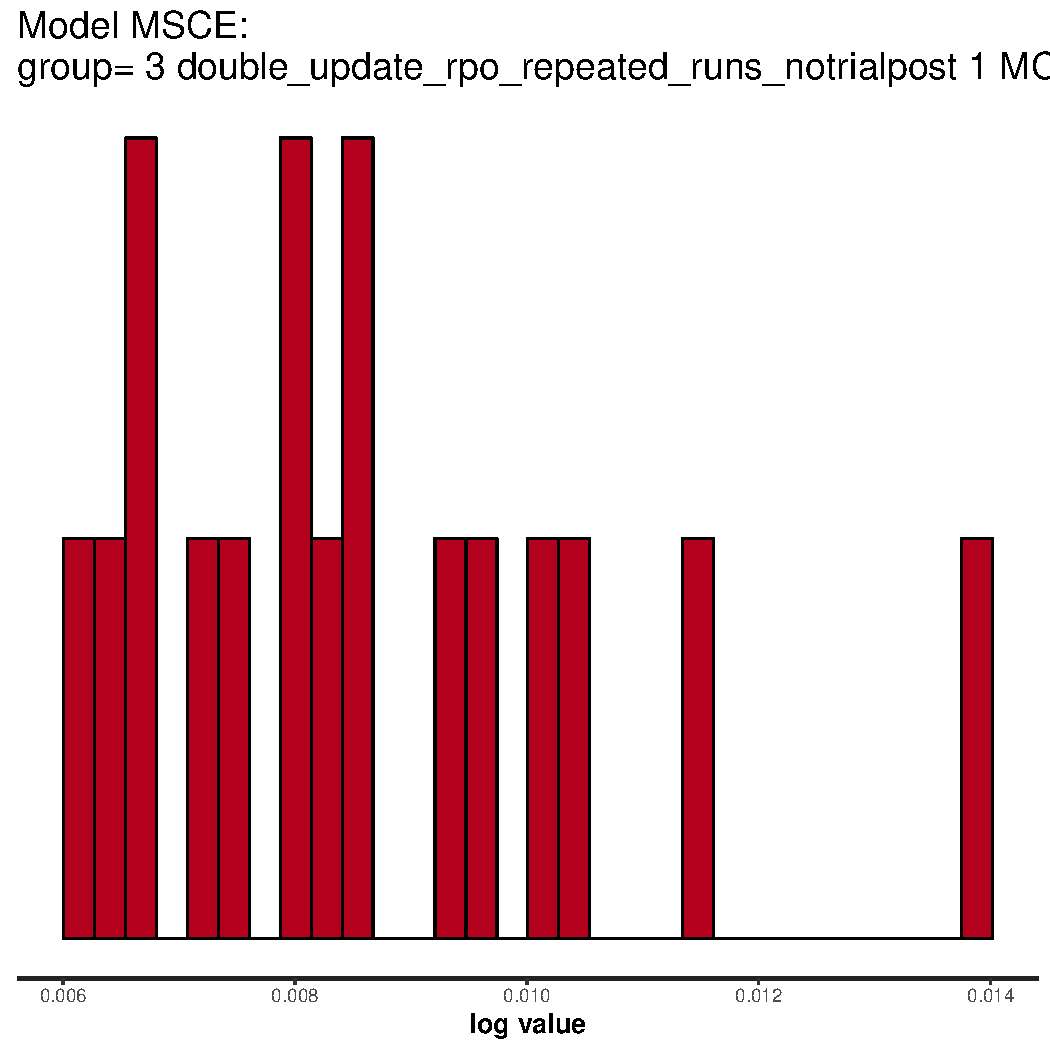
\includegraphics[width=\maxwidth]{figure/unnamed-chunk-12-4} 

\end{knitrout}

Autocorrelation, and effective sample size

\begin{knitrout}
\definecolor{shadecolor}{rgb}{0.969, 0.969, 0.969}\color{fgcolor}\begin{kframe}
\begin{verbatim}
## Inference for Stan model: double_update_notrialpost.
## 12 chains, each with iter=5000; warmup=1000; thin=1; 
## post-warmup draws per chain=4000, total post-warmup draws=48000.
## 
##           mean se_mean   sd  2.5%   25%   50%   75% 97.5% n_eff Rhat
## mu_p[1]  -0.57       0 0.17 -0.90 -0.68 -0.57 -0.45 -0.23 12321    1
## mu_p[2]  -1.10       0 0.05 -1.20 -1.13 -1.09 -1.06 -1.00 18692    1
## sigma[1]  1.17       0 0.16  0.89  1.05  1.15  1.27  1.53 24704    1
## sigma[2]  0.25       0 0.05  0.17  0.21  0.24  0.28  0.35 14660    1
## 
## Samples were drawn using NUTS(diag_e) at Mon Oct 16 21:52:58 2017.
## For each parameter, n_eff is a crude measure of effective sample size,
## and Rhat is the potential scale reduction factor on split chains (at 
## convergence, Rhat=1).
## 
## 
## Inference for Stan model: double_update_notrialpost.
## 12 chains, each with iter=5000; warmup=1000; thin=1; 
## post-warmup draws per chain=4000, total post-warmup draws=48000.
## 
##           mean se_mean   sd  2.5%   25%   50%   75% 97.5% n_eff Rhat
## mu_p[1]  -0.89       0 0.17 -1.23 -1.00 -0.89 -0.78 -0.56 13221    1
## mu_p[2]  -1.11       0 0.07 -1.25 -1.15 -1.11 -1.07 -0.99 20357    1
## sigma[1]  0.85       0 0.15  0.60  0.74  0.84  0.94  1.19 17606    1
## sigma[2]  0.18       0 0.07  0.05  0.14  0.18  0.23  0.34 10359    1
## 
## Samples were drawn using NUTS(diag_e) at Mon Oct 16 22:13:59 2017.
## For each parameter, n_eff is a crude measure of effective sample size,
## and Rhat is the potential scale reduction factor on split chains (at 
## convergence, Rhat=1).
## 
## 
## Inference for Stan model: double_update_rpo_repeated_runs_notrialpost.
## 12 chains, each with iter=5000; warmup=1000; thin=1; 
## post-warmup draws per chain=4000, total post-warmup draws=48000.
## 
##             mean se_mean   sd  2.5%   25%   50%   75% 97.5% n_eff Rhat
## mu_p[1,1]  -0.54       0 0.13 -0.80 -0.63 -0.54 -0.45 -0.29  8306    1
## mu_p[1,2]  -0.96       0 0.05 -1.05 -0.99 -0.96 -0.93 -0.87 16294    1
## mu_p[2,1]  -0.55       0 0.16 -0.88 -0.66 -0.55 -0.44 -0.23  8556    1
## mu_p[2,2]  -1.10       0 0.05 -1.21 -1.14 -1.10 -1.07 -1.01 16307    1
## sigma[1,1]  0.97       0 0.11  0.78  0.89  0.96  1.03  1.20 14388    1
## sigma[1,2]  0.26       0 0.04  0.19  0.23  0.26  0.29  0.36 16148    1
## sigma[2,1]  1.17       0 0.14  0.92  1.06  1.16  1.26  1.49 18061    1
## sigma[2,2]  0.25       0 0.05  0.17  0.22  0.25  0.28  0.35 14420    1
## 
## Samples were drawn using NUTS(diag_e) at Tue Oct 17 03:28:56 2017.
## For each parameter, n_eff is a crude measure of effective sample size,
## and Rhat is the potential scale reduction factor on split chains (at 
## convergence, Rhat=1).
## 
## 
## Inference for Stan model: double_update_rpo_repeated_runs_notrialpost.
## 12 chains, each with iter=5000; warmup=1000; thin=1; 
## post-warmup draws per chain=4000, total post-warmup draws=48000.
## 
##             mean se_mean   sd  2.5%   25%   50%   75% 97.5% n_eff Rhat
## mu_p[1,1]  -0.71       0 0.20 -1.11 -0.84 -0.71 -0.58 -0.33  9196    1
## mu_p[1,2]  -1.14       0 0.08 -1.30 -1.19 -1.13 -1.08 -0.99 11580    1
## mu_p[2,1]  -0.89       0 0.17 -1.22 -1.00 -0.88 -0.77 -0.56 15845    1
## mu_p[2,2]  -1.12       0 0.07 -1.25 -1.16 -1.11 -1.07 -1.00 26811    1
## sigma[1,1]  1.00       0 0.17  0.71  0.88  0.98  1.10  1.38 19298    1
## sigma[1,2]  0.30       0 0.08  0.15  0.25  0.30  0.35  0.47  7661    1
## sigma[2,1]  0.86       0 0.14  0.62  0.76  0.84  0.94  1.18 23980    1
## sigma[2,2]  0.19       0 0.07  0.06  0.14  0.18  0.23  0.34 11069    1
## 
## Samples were drawn using NUTS(diag_e) at Tue Oct 17 08:35:26 2017.
## For each parameter, n_eff is a crude measure of effective sample size,
## and Rhat is the potential scale reduction factor on split chains (at 
## convergence, Rhat=1).
\end{verbatim}
\end{kframe}
\end{knitrout}
Effective sample sizes are now sensible.
\begin{knitrout}
\definecolor{shadecolor}{rgb}{0.969, 0.969, 0.969}\color{fgcolor}\begin{kframe}
\begin{verbatim}
## [1] TRUE
\end{verbatim}
\end{kframe}
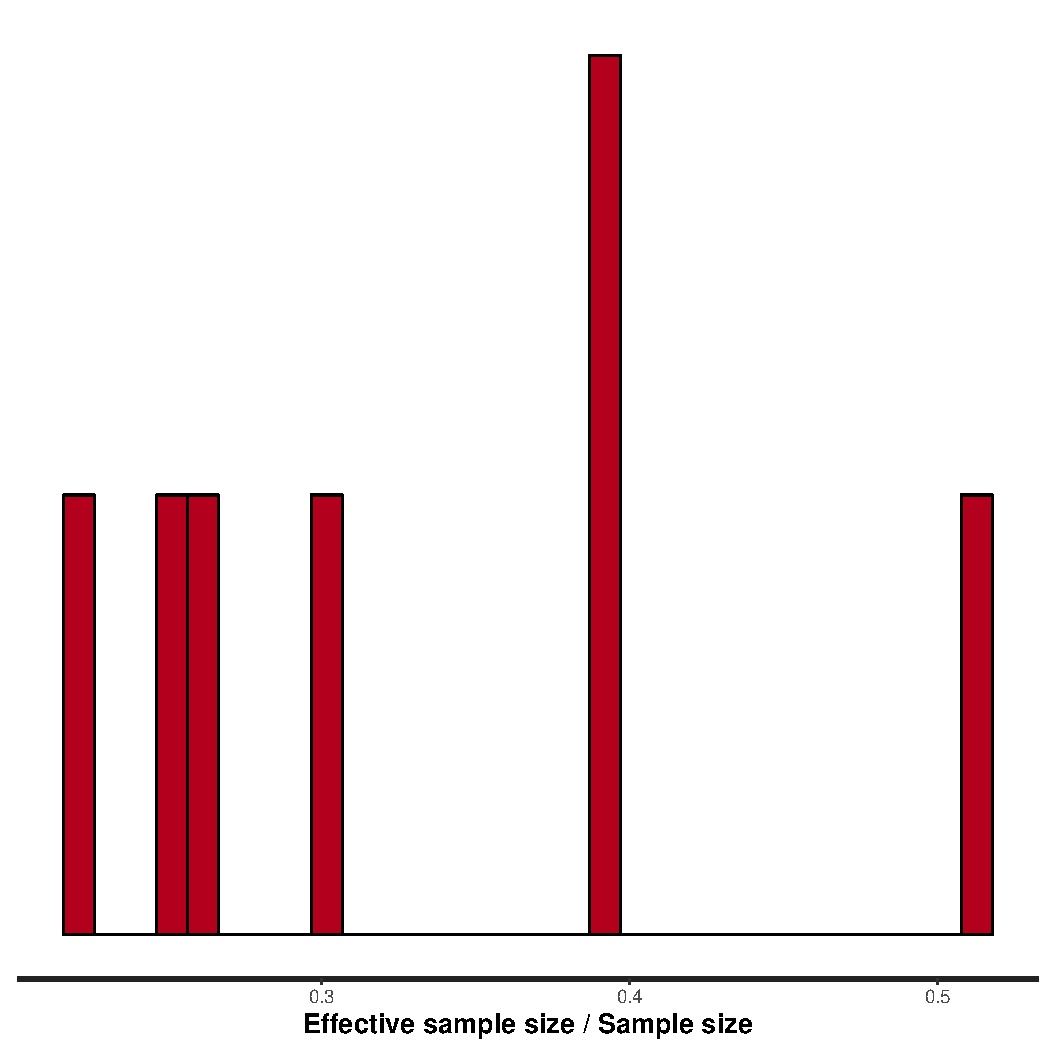
\includegraphics[width=\maxwidth]{figure/unnamed-chunk-14-1} 
\begin{kframe}\begin{verbatim}
## [1] TRUE
\end{verbatim}
\end{kframe}
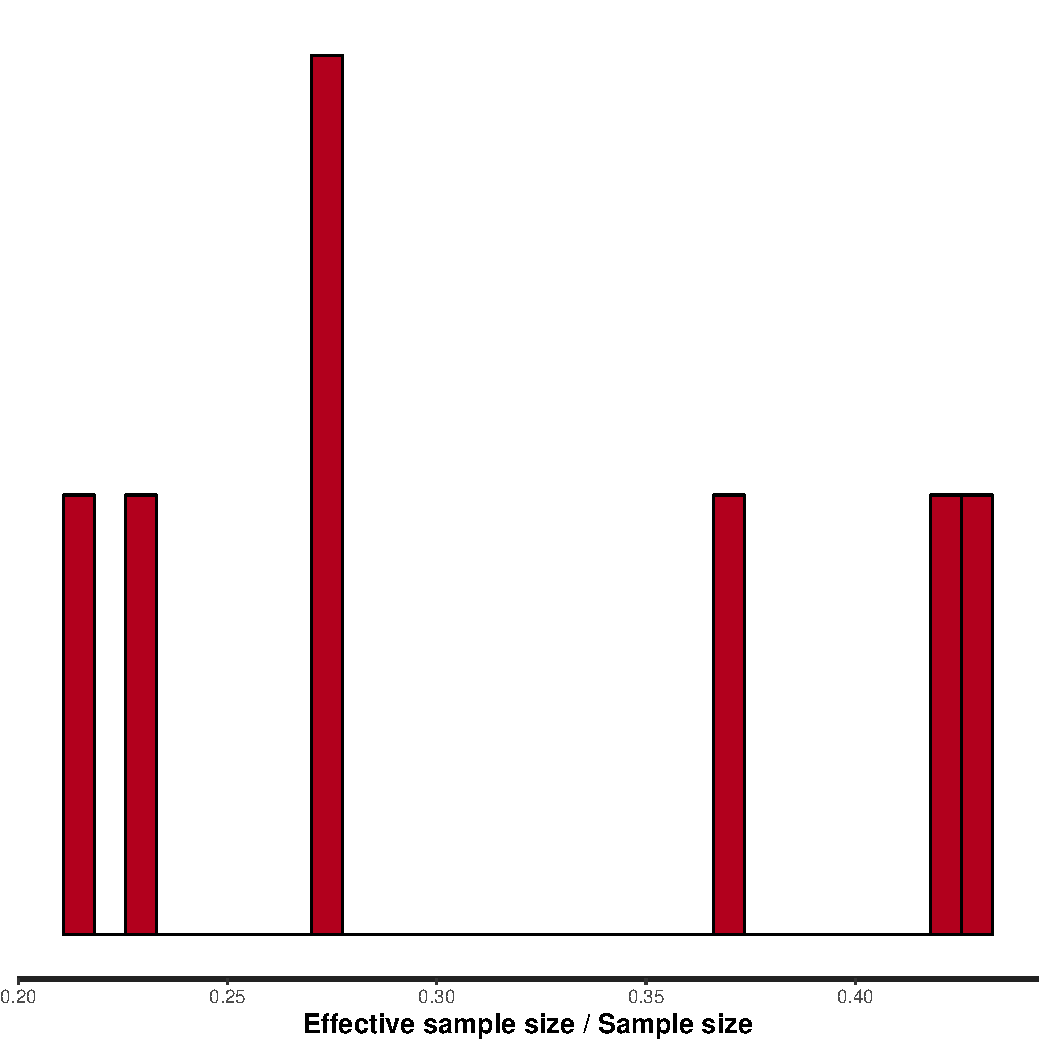
\includegraphics[width=\maxwidth]{figure/unnamed-chunk-14-2} 
\begin{kframe}\begin{verbatim}
## [1] FALSE
\end{verbatim}
\end{kframe}
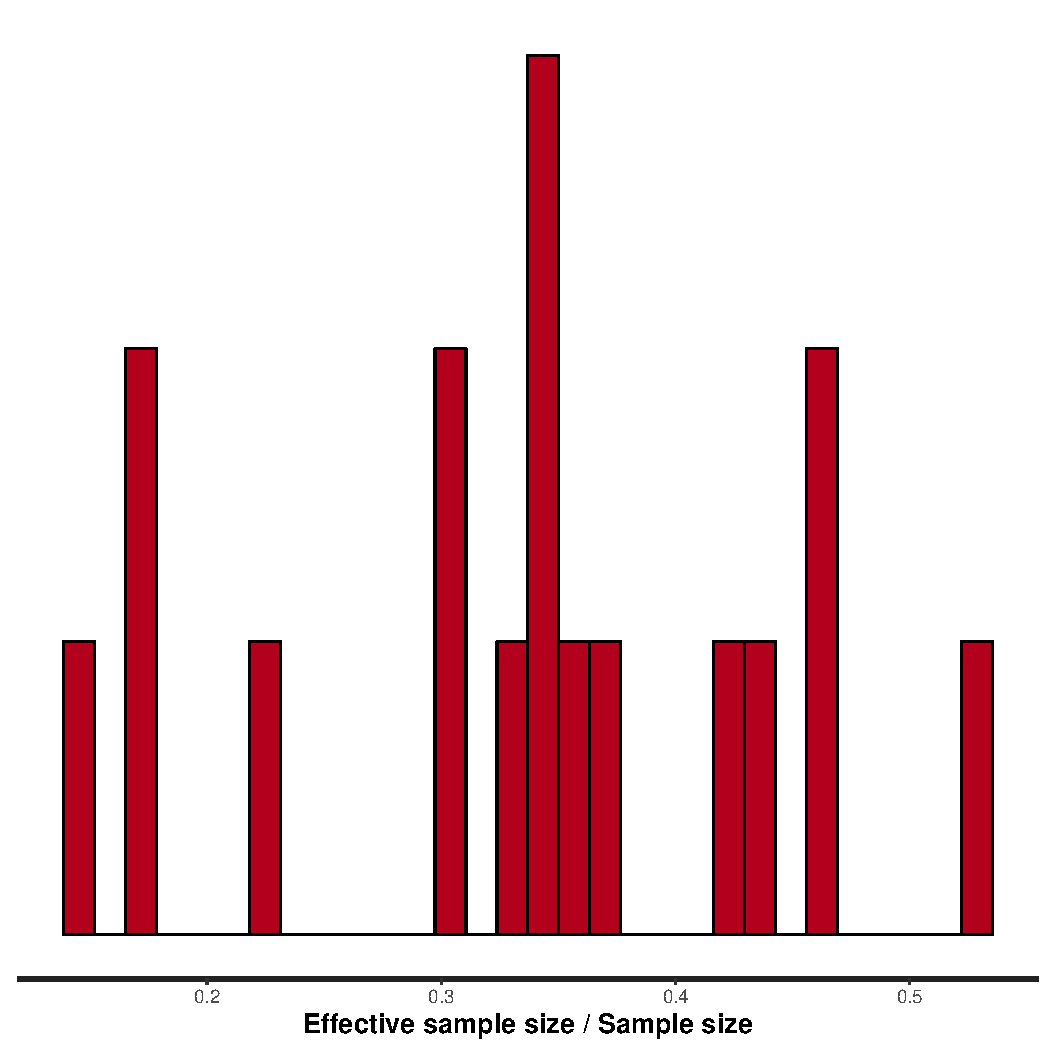
\includegraphics[width=\maxwidth]{figure/unnamed-chunk-14-3} 
\begin{kframe}\begin{verbatim}
## [1] FALSE
\end{verbatim}
\end{kframe}
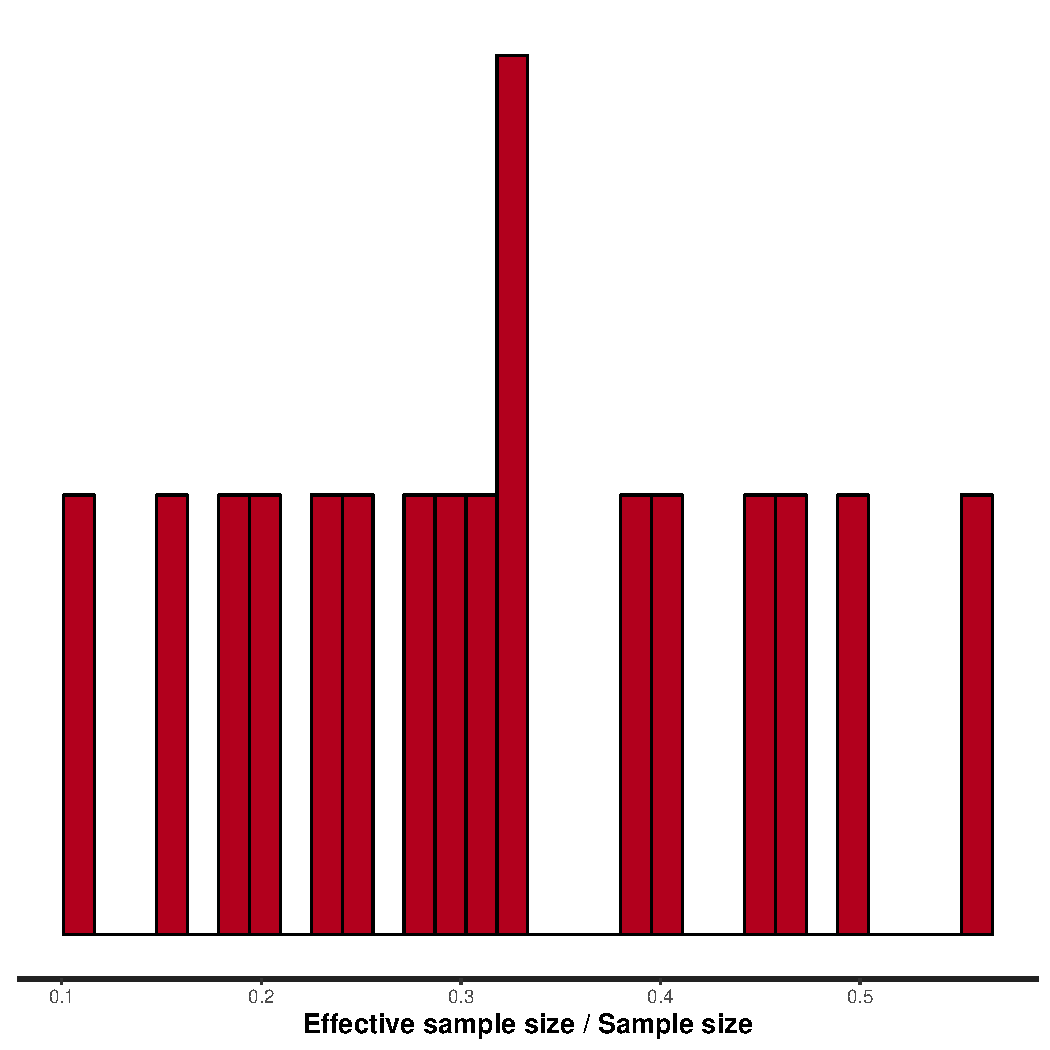
\includegraphics[width=\maxwidth]{figure/unnamed-chunk-14-4} 

\end{knitrout}

\section*{Discussion}

Overall, we could not find differences between groups in overall performance. We did find evidence that inverse temperature differs for subjects--for both groups--between reward and punishment rounds. This is something to look into further.

Next steps:
\begin{itemize}
  \item Look into the inverse temperature difference more closely. Can we validate that this is a real effect, and why would this be?
  \item Compare Safe No Meth with Safe Meth users
  \item See if we can get more precise posteriors with DE-MCMC
  \item Try to integrate neural data from the pain classifier or other sources
\end{itemize}

\end{document}
